
\section{Multithreading}


Tråde er er programstykker som kan eksekveres parallelt med hinanden, dvs. "på samme tid". På single-core systemer skifter operativsystemet konstant mellem trådene, hvilket giver illusionen af, at de kører parallelt. På multi-core systemer kan operativsystemet derimod virkelig afvikle tråde parallelt - én på hver core.

\subsection{Fordele}

\begin{itemize}
  \item Gør det muligt at separere program-kode fra kontrol-kode, fx kan lange rekursive beregninger udføres i én tråd, mens main-tråden fortsat reagerer på inputs fra brugeren.
  \item Kan således forhindre at programmer "fryser" mens lange beregninger finder sted.
\end{itemize}

\subsection{Ulemper}

\begin{itemize}
  \item Der kan opstå problemer, fx race conditions ved synkronisering hvis flere tråde deler data.
  \item Deadlocks hvis alle aktive tråde venter på at nogle andre tråde "gør noget"
\end{itemize}

\subsection{Runnable interfacet}

\begin{itemize}
  \item En class som implementerer Runnable interfacet skal override metoden run(), hvorefter et Thread-objekt kan laves med et objekt af denne "Runnable class". Herefter kaldes start() på Thread-objektet, og så afvikles koden i Runnable objektets run() metode.
  \begin{verbatim}
    Runnable r = new MyRunnable();
    Thread t = new Thread(r);
    t.start();
  \end{verbatim}
  \item UML diagram
  
  \begin{center}
    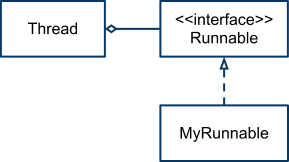
\includegraphics[scale=0.6]{images/runnable_uml.png}
  \end{center}
    
\end{itemize}

\subsection{Selfishness}

\begin{itemize}
  \item En tråd skal lade andre tråde "komme til", ellers er den selfish. På nogle platforme kan en selfish tråd forhindre andre tråde i at blive afviklet, hvilket ødelægger formålet med tråde.
  \item Tråde kan sættes til at "sove" med sleep(). Når en tråd sættes til at sove betyder det, at andre tråde kan komme til.
  \item En tråds afviklingstid kaldes en "time slice".
  \begin{itemize}
    \item main() metoden i ethvert Java program er sin egen tråd.
    \item Hvis man har startet flere tråde i sit program afsluttes det først når alle trådene er færdige, eller er blevet interrupted.
  \end{itemize}
\end{itemize}

\subsection{Tilstand}

\begin{itemize}
  \item Diagram
  
  \begin{center}
    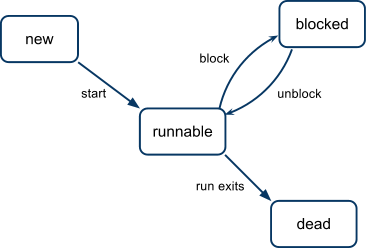
\includegraphics[scale=0.7]{images/thread_states.png}
  \end{center}
    
  \begin{itemize}
    \item Når der laves et nyt Thread objekt er den new. Når \verb start() metoden kaldes bliver tråden runnable. Herfra er tråden klar til at blive kørt. Tråden kan blive blocked hvis der kaldes \verb wait() eller \verb sleep(). Dette sker som regel når tråden venter på en lås. Når tråden vækkes af enten \verb notify() eller \verb signal() bliver den igen runnable. Når \verb run() metoden returnerer dør tråden.
  \end{itemize}

  \item En tråd kan være blocked hvis den sover, venter på input/output, venter på en lock eller en condition.
  \item Når en tråd er blocked forbliver den blocked indtil den event den venter på sker. Fx, hvis en tråd sover bliver den først runnable igen når dens sovetid er gået.
\end{itemize}

\subsection{interrupt()}

\begin{itemize}
  \item Tråde kan afbrydes/stoppes med \verb|interrupt()| 
  \item sleep() og wait() kaster en InterruptedException, hvis interupt() kaldes på en "sovende tråd". Denne exception skal fanges, og man bør derfor omringe al koden i run() med en try-blok.
  \item Hvis tråden ikke er blocked vil interrupt() bare sætte trådens interrupted field til true. Dette field kan checkes med metoden isInterrupted().
  \item I tilfælde af I/O eller andet "beskidt" arbejde bør tråde altid have noget oprydningskode efter try-blokken.
\end{itemize}

\subsection{Race conditions}

\begin{itemize}
  \item Når flere tråde deler data, som kan korrupteres hvis trådene ikke afvikles i en bestemt rækkefølge.
  \item Hvis to tråde fx forsøger at lægge nyt indhold i en queue, og samtidig inkrementerer queuens tail, så kan race conditions gøre, at en tråd ikke når at inkrementere tailen før en ny tråd tager over. I så fald overskrives den første tråds data. Se evt. Horstmann s. 376
  \item Locks kan bruges til at blokkere alle andre tråde, som forsøger at tilgå den samme data som den nuværende tråd, indtil denne er færdig med sin kode. Når den første tråd frigiver locken, bliver de andre tråde unblocked.
  \begin{itemize}
    \item En tråd kan "acquire" en lock ved at kalde lock() på locken. Hvis en anden tråd forsøger at acquire en locked lock bliver den blocked, indtil den første tråd kalder unlock() på locken.
    \item Locks sikrer, at en tråd færdiggør sit arbejde med noget data før eventuelle andre tråde kan korruptere det.
  \end{itemize}

  \item Deadlocks - når ingen tråde kan fortsætte fordi de venter på at en anden tråd gør noget først. Fx hvis en tråd venter på at der bliver plads i en fuld queue, men queuen ikke bliver tømt, da ingen tråde kan få locken, så de kan fjerne elementer fra queuen.
  \begin{itemize}
    \item En lock kan have et tilknyttet Condition objekt. Hvis man kalder await() på et Condition objekt kan man lade andre tråde få den lock som den nuværende tråd har.
    \item En tråd, som har kaldt await() på et tilhørende Condition objekt er blokkeret indtil en anden tråd kalder signalAll() på Condition objektet som tråden venter på.
    \item Typisk laves checks på Condition objekter i while-løkker, \\
    fx \verb|while (not OK to proceed) Condition.await()|
  \end{itemize}

  \item Der er object locks bygget ind i alle Java objekter. Disse kan bruges på samme måde som ReentrantLocks, men i stedet for at opsætte locks skal synkroniserede metoder tagges med "synchronized" keywordet, fx "\verb|public synchronized void add(E newValue)|".
  \begin{itemize}
    \item Når en synchronized metode kaldes låses object locken.
    \item Når en synchronized metode er færdig frigives object locken.
    \item Object locks har én (anonym) Condition.
    \item \verb|wait() <-> await()| og \verb|notifyAll() <-> signalAll()|, dvs. man kan frigive object locken på næsten samme måde som med ReentrantLock, og ligeledes signalere til alle ventende tråde.
  \end{itemize}

  \item java.util.concurrent biblioteket har en BlockingQueue klasse, som er designet med race conditions i baghovedet. Queuens put() og take() metoder afventer på hhv. plads i køen og elementer i køen, før de fortsætter.
  \begin{itemize}
    \item Concurrent = samtidig
  \end{itemize}

\end{itemize}


